% greens_guide.tex
\documentclass[11pt]{article}

% ---------- Preamble ----------
\usepackage[margin=1.05in]{geometry}
\usepackage[T1]{fontenc}
\usepackage{lmodern}
\usepackage{microtype}
\usepackage{amsmath,amssymb,amsthm,mathtools}
\usepackage{bm}
\usepackage{physics}
\usepackage{upquote}
\usepackage{enumerate}
\usepackage{tikz}
\usepackage{graphicx}
\usepackage{caption}
\usepackage[colorlinks=true,linkcolor=blue!60!black,citecolor=blue!60!black,urlcolor=blue!60!black]{hyperref}
\usepackage[nameinlink,noabbrev]{cleveref}
\setlength{\parskip}{6pt}
\setlength{\parindent}{0pt}

% ---------- Theorem styles ----------
\newtheorem{theorem}{Theorem}[section]
\newtheorem{proposition}[theorem]{Proposition}
\newtheorem{lemma}[theorem]{Lemma}
\newtheorem{corollary}[theorem]{Corollary}
\theoremstyle{definition}
\newtheorem{definition}[theorem]{Definition}
\newtheorem{example}[theorem]{Example}
\theoremstyle{remark}
\newtheorem{remark}[theorem]{Remark}

% ---------- Shortcuts ----------
\newcommand{\R}{\mathbb{R}}
\newcommand{\C}{\mathbb{C}}
\newcommand{\D}{\mathbb{D}}
\newcommand{\Om}{\Omega}
\newcommand{\ol}{\overline}
\DeclareMathOperator{\divg}{div}
\DeclareMathOperator{\spt}{spt}
\DeclarePairedDelimiter{\ang}{\langle}{\rangle}

% A neat box for key formulas
\usepackage[most]{tcolorbox}
\tcbset{colback=white,colframe=black!15,left=6pt,right=6pt,top=6pt,bottom=6pt,boxsep=0pt}

% ---------- Title ----------
\title{When Closed Forms Exist (and How to Get Them):\\
	Green's Functions, Fundamental Solutions, and Classic Constructions}
\author{Prepared for internal wiki / Electron export}
\date{\today}

\begin{document}
	\maketitle
	
	\tableofcontents
	
	\section{Green's functions in the distributional sense}
	
\begin{definition}[Fundamental solution]
	Let $L$ be a linear differential operator on $\mathbb{R}^n$. 
	A \emph{fundamental solution} $\Phi$ satisfies $L\Phi=\delta$ in the sense of distributions: 
	for all $\varphi\in C_c^\infty(\mathbb{R}^n)$,
	\[
	\ang{\Phi, L^*\varphi}=\varphi(0),
	\]
	where $L^*$ is the formal adjoint of $L$.
\end{definition}

\begin{definition}[Green's function on a domain]
	For a bounded domain $\Omega\subset\mathbb{R}^n$ with boundary condition $B$ (e.g.\ Dirichlet 
	$u|_{\partial\Omega}=0$ or Neumann $\partial_\nu u|_{\partial\Omega}=0$), a Green's function $G(\cdot,\xi)$ solves
	\[
	L\,G(\cdot,\xi)=\delta_\xi \quad\text{in }\Omega,\qquad
	B\,G(\cdot,\xi)=0\quad\text{on }\partial\Omega.
	\]
\end{definition}
	
	\paragraph{Representation formula.}
	If $G$ exists and $u$ solves $Lu=f$ in $\Om$ with boundary data matching $B$, then
	\[
	u(x)=\int_\Om G(x,\xi)f(\xi)\,d\xi + \text{(boundary layer term depending on $B$)}.
	\]
	For homogeneous Dirichlet, the boundary term vanishes.
	
	\paragraph{Jump condition in 1D.}
	If $L=-(p y')'+q y$ on $(a,b)$ and $G(\cdot,\xi)$ satisfies $L G(\cdot,\xi)=\delta_\xi$,
	then $G$ is continuous at $x=\xi$ and its flux has a unit jump:
	\[
	p(\xi)\,\partial_x G(\xi^+,\xi)-p(\xi)\,\partial_x G(\xi^-,\xi)=1.
	\]
	
	\section{1D Sturm--Liouville: constructive recipe}
	
	Consider the self-adjoint operator
	\[
	Ly=-(p y')'+q y,\qquad p>0,\ q\ \text{real},\quad x\in(a,b),
	\]
	with self-adjoint boundary conditions (Dirichlet/Neumann/Robin at $a,b$).
	
	\begin{tcolorbox}
		\textbf{Construction.} Let $u_{<}$ solve $Lu=0$ satisfying the left boundary condition at $x=a$,
		and let $u_{>}$ solve $Lu=0$ satisfying the right boundary condition at $x=b$.
		The Wronskian
		\[
		W(x)=p(x)\big(u_{<}u_{>}'-u_{<}'u_{>}\big)
		\]
		is constant $\,(=W)\,$ on $(a,b)$. Then
		\[
		G(x,\xi)=\frac{1}{W}\begin{cases}
			u_{<}(x)\,u_{>}(\xi), & x\le \xi,\\[2pt]
			u_{<}(\xi)\,u_{>}(x), & x\ge \xi.
		\end{cases}
		\]
	\end{tcolorbox}
	
	\begin{example}[Dirichlet Poisson on $(0,1)$]
		$Ly=-y''$, $u(0)=u(1)=0$. Solutions of $Lu=0$ with the left/right BC are $u_{<}(x)=x$ and
		$u_{>}(x)=1-x$, giving $W=1$. Thus
		\[
		G(x,\xi)=\min(x,\xi)\big(1-\max(x,\xi)\big)
		=\begin{cases}x(1-\xi),&x\le\xi,\\ \xi(1-x),&x\ge\xi.\end{cases}
		\]
	\end{example}
	
	\begin{example}[Dirichlet with $Ly=-y''$ on $(0,1)$ but hyperbolic basis]
		Setting $u_{<}=\sinh x$, $u_{>}=\sinh(1-x)$ also yields $W=\sinh 1$, hence
		\[
		G(x,\xi)=\frac{1}{\sinh 1}\begin{cases}
			\sinh x\,\sinh(1-\xi),&x\le \xi,\\
			\sinh \xi\,\sinh(1-x),&x\ge \xi.
		\end{cases}
		\]
	\end{example}
	
	\begin{remark}[Robin and Neumann]
		For Robin $a_0 u + a_1 p u' = 0$ at an endpoint, pick $u_{<},u_{>}$ to satisfy those mixed
		conditions. The same Wronskian formula applies; only $W$ changes.
	\end{remark}
	
	\section{Free-space fundamental solutions in $\R^n$}
	
	Let $r=\abs{x}$ and $H_0^{(1)}$ be the Hankel function.
	
	\begin{tcolorbox}
		\textbf{Laplace} $-\Delta\Phi=\delta$:
		\[
		\Phi_n(x)=\begin{cases}
			\dfrac{1}{(n-2)\omega_n}\,r^{2-n}, & n\ge3,\\[8pt]
			-\dfrac{1}{2\pi}\log r, & n=2,
		\end{cases}
		\quad\ \omega_n=\text{surface area of }S^{n-1}=\dfrac{2\pi^{n/2}}{\Gamma(n/2)}.
		\]
	\end{tcolorbox}
	
	\begin{tcolorbox}
		\textbf{Helmholtz} $(\Delta+k^2)\Phi=\delta$ (outgoing):
		\[
		\Phi_3(x)=\frac{e^{ik r}}{4\pi r},\qquad
		\Phi_2(x)=\frac{i}{4}\,H_0^{(1)}(k r).
		\]
	\end{tcolorbox}
	
	\begin{remark}
		These are distributional identities; away from $r=0$ the kernels are classical solutions.
		The singularity encodes the point source.
	\end{remark}
	
	\section{Method of images}
	
	For domains with simple symmetries, combine free-space kernels with \emph{images} that enforce
	boundary conditions.
	
	\paragraph{Half-space Dirichlet for Laplace (3D).} For $\Om=\{x_3>0\}$, Dirichlet data $u|_{x_3=0}=0$:
	\[
	G(x,\xi)=\frac{1}{4\pi}\bigg(\frac{1}{\abs{x-\xi}}-\frac{1}{\abs{x-\xi^\ast}}\bigg),
	\quad \xi^\ast=(\xi_1,\xi_2,-\xi_3).
	\]
	Neumann uses a plus sign.
	
	\paragraph{Sphere (Kelvin transform).} For a ball, the image point is at the inversion point and
	a scaling is needed; the same idea applies with a modified coefficient.
	
	\section{Conformal mapping in 2D}
	
	If $\phi:\Om\to\Om'$ is conformal and $G_{\Om'}$ is the Dirichlet Green's function on $\Om'$,
	then
	\[
	G_\Om(z,\xi)=G_{\Om'}\big(\phi(z),\phi(\xi)\big)
	\]
	because the Laplacian is conformally invariant up to a Jacobian that cancels in the Green
	identity for Dirichlet problems.
	
	\begin{tcolorbox}
		\textbf{Unit disk Dirichlet kernel.}
		For $\D=\{z:|z|<1\}$,
		\[
		G_{\D}(z,\xi)=-\frac{1}{2\pi}\log\abs{\frac{z-\xi}{1-\ol{\xi}\,z}}.
		\]
	\end{tcolorbox}
	
	\begin{example}[Upper half-plane]
		Map $\mathbb{H}=\{\Im z>0\}$ to $\D$ by the Cayley transform
		$\phi(z)=\dfrac{z-i}{z+i}$. Then
		\[
		G_{\mathbb{H}}(z,\xi)=G_{\D}\!\big(\phi(z),\phi(\xi)\big)
		=-\frac{1}{2\pi}\log\abs{\frac{z-\xi}{z-\ol{\xi}}}.
		\]
		This equals the method-of-images kernel for the line boundary.
	\end{example}
	
	\section{Existence, uniqueness, and the Green identity}
	
	\begin{theorem}[Uniqueness for Dirichlet Poisson]
		Let $\Om$ be bounded with $C^{1}$ boundary. For $Lu=-\Delta u$ with Dirichlet data,
		the Green's function is unique, symmetric $G(x,\xi)=G(\xi,x)$, and
		\[
		u(x)=\int_\Om G(x,\xi) f(\xi)\,d\xi
		\]
		is the unique weak solution in $H_0^1(\Om)$ for $f\in H^{-1}(\Om)$.
	\end{theorem}
	
	\begin{proof}[Sketch]
		Lax–Milgram yields existence/uniqueness in $H_0^1$. Symmetry follows from self-adjointness
		and the reciprocity identity $\int G(x,\xi)f(\xi)d\xi=\int G(\xi,x)f(\xi)d\xi$ for all $f$.
	\end{proof}
	
	\paragraph{Weak formulation.}
	For $f\in H^{-1}(\Om)$, $u\in H_0^1(\Om)$ solves $-\Delta u=f$ iff
	\[
	\int_\Om \nabla u\cdot \nabla \varphi\,dx = \ang{f,\varphi}\quad \forall\,\varphi\in H_0^1(\Om).
	\]
	With $G$, testing against $\varphi(\cdot)=G(\cdot,\xi)$ reproduces the representation.
	
	
	
	\section{Eigenfunction expansions on bounded domains}
	\label{sec:eigexp}
	
	Let $\Omega\subset\mathbb{R}^n$ be bounded with sufficiently regular boundary and let
	\[
	L u := -\divg(A\nabla u)+c\,u
	\]
	be a uniformly elliptic, real, self-adjoint operator on $H_0^1(\Omega)$ (Dirichlet) or on
	$H^1(\Omega)$ with Neumann/Robin boundary conditions. Assume $A(x)$ is symmetric, bounded,
	and uniformly positive definite, $c\in L^\infty(\Omega)$ with $c\ge 0$.
	
	\begin{theorem}[Spectral theorem (compact resolvent)]
		There exists an orthonormal basis $\{\phi_k\}_{k=1}^\infty$ of $L^2(\Omega)$ consisting of
		eigenfunctions of $L$,
		\[
		L\phi_k=\lambda_k \phi_k,\qquad 0<\lambda_1\le \lambda_2\le \cdots,\ \ \lambda_k\to\infty,
		\]
		for Dirichlet (and $\lambda_1=0$ may occur for Neumann/Robin, with $\phi_1$ constant when $c\equiv0$).
		The eigenfunctions are in $H^2(\Omega)$ (and smooth if $A,c,\partial\Omega$ are smooth).
	\end{theorem}
	
	\paragraph{Green series.}
	For Dirichlet (or after removing the nullspace for Neumann/Robin), the Green's function admits
	the \emph{eigenfunction expansion}
	\begin{equation}
		\label{eq:Gseries}
		G(x,\xi)=\sum_{k=1}^\infty \frac{\phi_k(x)\,\phi_k(\xi)}{\lambda_k},
	\end{equation}
	converging in $L^2(\Omega\times\Omega)$ and, away from the diagonal $x=\xi$, locally uniformly.
	Termwise application of $L$ gives $LG(\cdot,\xi)=\delta_\xi$ in the distributional sense.
	
	\begin{remark}[Neumann/Robin zero mode]
		If $0$ is an eigenvalue (e.g.\ Neumann with $c\equiv0$), use the \emph{reduced Green's function}
		by projecting off the nullspace:
		\[
		G(x,\xi)=\sum_{\lambda_k>0}\frac{\phi_k(x)\phi_k(\xi)}{\lambda_k}.
		\]
		The representation of solutions then holds for data orthogonal to the nullspace (e.g.\ zero-mean $f$ for Neumann Laplacian).
	\end{remark}
	
	\begin{example}[Rectangle, Dirichlet Laplacian]
		$\Omega=(0,a)\times(0,b)$, $L=-\Delta$, $u|_{\partial\Omega}=0$. The eigenpairs are
		\[
		\phi_{mn}(x,y)=\frac{2}{\sqrt{ab}}\sin\!\frac{m\pi x}{a}\ \sin\!\frac{n\pi y}{b},\qquad
		\lambda_{mn}=\Big(\frac{m\pi}{a}\Big)^2+\Big(\frac{n\pi}{b}\Big)^2,\quad m,n\in\mathbb{N}.
		\]
		Hence
		\[
		G(x,\xi)=\sum_{m,n\ge1}\frac{\phi_{mn}(x)\,\phi_{mn}(\xi)}{\lambda_{mn}}.
		\]
		This is a sine series; for strips and intervals the sum collapses to closed forms with $\sinh/\cosh$.
	\end{example}
	
	\begin{example}[Disk, Dirichlet Laplacian]
		In polar coordinates, the eigenfunctions are $J_{|m|}(j_{|m|,k} r/R)e^{im\theta}$,
		with $\lambda_{m,k}=j_{|m|,k}^2/R^2$ (zeros of Bessel $J_{|m|}$). Then
		\[
		G(r,\theta;\rho,\vartheta)=\sum_{m\in\mathbb{Z}}\sum_{k\ge1}
		\frac{J_{|m|}(j_{|m|,k}r/R)J_{|m|}(j_{|m|,k}\rho/R)}{\lambda_{m,k}\, \pi R^2 [J_{|m|+1}(j_{|m|,k})]^2}
		\,e^{im(\theta-\vartheta)}.
		\]
	\end{example}
	
	\begin{remark}[Convergence and regularity]
		The series \eqref{eq:Gseries} converges absolutely on compact subsets of $\{(x,\xi):x\neq \xi\}$
		and reproduces the logarithmic (2D) or Newtonian ($n\ge3$) singularity as $x\to\xi$.
		Smoothing $f$ increases convergence rate of the represented solution
		$u(x)=\int_\Omega G(x,\xi)f(\xi)\,d\xi$ by eigen-coefficient decay.
	\end{remark}
	
	\section{Transform methods for translation-invariant problems}
	\label{sec:transforms}
	
	On $\mathbb{R}^n$ (or tori with periodic boundary conditions), many operators are \emph{convolution}
	operators, diagonalized by the Fourier transform.
	
	\paragraph{Conventions.}
	For $u\in\mathcal{S}(\mathbb{R}^n)$,
	\[
	\widehat{u}(k)=\int_{\mathbb{R}^n} e^{-ik\cdot x}u(x)\,dx,\qquad
	u(x)=\frac{1}{(2\pi)^n}\int_{\mathbb{R}^n} e^{ik\cdot x}\widehat{u}(k)\,dk.
	\]
	If $L$ has constant coefficients, its \emph{symbol} $L(k)$ satisfies
	$\widehat{Lu}(k)=L(k)\,\widehat{u}(k)$.
	
	\begin{tcolorbox}
		\textbf{Green kernel via symbol.}
		If $L(k)$ has no zeros (or after choosing a distributional prescription at zeros),
		the free-space Green's function is
		\[
		\widehat{G}(k)=\frac{1}{L(k)},\qquad
		G(x)=\frac{1}{(2\pi)^n}\int_{\mathbb{R}^n}\frac{e^{ik\cdot x}}{L(k)}\,dk,
		\]
		interpreted as an oscillatory integral (tempered distribution).
	\end{tcolorbox}
	
	\begin{example}[Laplace]
		$L=-\Delta\ \Rightarrow\ L(k)=|k|^2$. Then
		\[
		G(x)=\mathcal{F}^{-1}\!\Big(\frac{1}{|k|^2}\Big)=
		\begin{cases}
			\dfrac{1}{(n-2)\omega_n}\,|x|^{2-n}, & n\ge3,\\[8pt]
			-\dfrac{1}{2\pi}\log|x|, & n=2,
		\end{cases}
		\]
		reproducing the fundamental solutions.
	\end{example}
	
	\begin{example}[Helmholtz and radiation condition]
		$L=\Delta+k_0^2\ \Rightarrow\ L(k)=-(|k|^2-k_0^2)$. The inverse requires a causal/outgoing
		prescription:
		\[
		\widehat{G}(k)=\frac{-1}{|k|^2-k_0^2-i0}.
		\]
		Taking the inverse transform yields the outgoing kernels
		$G_3(x)=\dfrac{e^{ik_0|x|}}{4\pi|x|}$ and
		$G_2(x)=\dfrac{i}{4}H_0^{(1)}(k_0|x|)$.
	\end{example}
	
	\begin{example}[Heat kernel (time domain)]
		For $u_t-\Delta u=\delta_{t=0}\delta_{x=0}$, the space--time Fourier transform gives
		$\widehat{G}(k,\omega)=\dfrac{1}{-i\omega+|k|^2}$, hence
		\[
		G(t,x)=\frac{\mathbf{1}_{t>0}}{(4\pi t)^{n/2}}\,e^{-\frac{|x|^2}{4t}}.
		\]
	\end{example}
	
	\begin{remark}[Periodic domains]
		On the torus $\mathbb{T}^n$, the spectrum is discrete: $k\in\mathbb{Z}^n$. Replace integrals by
		Fourier series,
		\[
		G(x)=\sum_{k\in\mathbb{Z}^n\setminus\{0\}}\frac{e^{ik\cdot x}}{L(k)},
		\]
		with the $k=0$ mode removed when necessary (e.g.\ Laplacian on $\mathbb{T}^n$).
	\end{remark}
	
	\begin{remark}[Regularization at zeros]
		If $L(k)$ vanishes (Laplace at $k=0$, Helmholtz on the sphere $|k|=k_0$), define
		$1/L(k)$ as a tempered distribution by limiting absorption ($\pm i0$), principal value,
		or by projecting off the nullspace; the physical choice is fixed by boundary/radiation conditions.
	\end{remark}
	
	\paragraph{Summary.}
	For translation-invariant operators, the transform route yields $G$ in one line via $1/L(k)$.
	For bounded/curved domains, combine free-space $G$ with images, boundary integral equations,
	or eigenfunction expansions from \Cref{sec:eigexp}.
	
	
	
	\section{How to select a construction (practical playbook)}
	
	\begin{enumerate}[(1)]
		\item \textbf{1D with separated BCs:} use the Sturm–Liouville recipe; two homogeneous bases + Wronskian.
		\item \textbf{Simple \emph{flat} boundaries (planes):} start from free-space kernel and enforce BCs by images.
		\item \textbf{2D \emph{smooth} simply-connected domains:} conformally map to the disk or half-plane and pull back
		the disk kernel.
		\item \textbf{Helmholtz/Time-harmonic:} pick the \emph{outgoing} free-space $\Phi$ (Sommerfeld radiation condition);
		use images only when symmetry/planarity allows.
	\end{enumerate}
	
	\section{Worked micro-examples}
	
	\begin{example}[Poisson on $(0,1)$ with $f\equiv1$]
		Using the Dirichlet $G$ from \S2,
		\[
		u(x)=\int_0^1 G(x,\xi)\,d\xi=\frac12 x(1-x).
		\]
	\end{example}
	
	\begin{example}[Half-space electrostatics]
		For a unit point charge at $\xi$ above a grounded plane $x_3=0$, the potential is
		$u(x)=G(x,\xi)$ from \S4. Field lines and image charge at $\xi^\ast$ satisfy Gauss law and zero trace.
	\end{example}
	
	\section{Numerical notes (for viewers and plotting)}
	
	\begin{itemize}
		\item In 2D, treat the logarithmic singularity by subtracting/adding $-\frac{1}{2\pi}\log|x-\xi|$
		and integrating the smooth remainder; or integrate in polar coordinates around $\xi$.
		\item For Helmholtz in 2D, avoid evaluating $H_0^{(1)}$ too near $0$; use series expansions or
		asymptotics depending on $k r$.
		\item In 1D plots, enforce the continuity of $G$ and the unit jump in $p\,\partial_x G$ at $x=\xi$.
	\end{itemize}
	
	\appendix
	\section{Quick kernel table}
	\begin{center}
		\begin{tabular}{|c|c|}
			\hline
			\textbf{Operator / Domain} & \textbf{Green / Fundamental solution}\\
			\hline
			$-\Delta$ in $\R^3$ & $\displaystyle \frac{1}{4\pi r}$\\
			\hline
			$-\Delta$ in $\R^2$ & $\displaystyle -\frac{1}{2\pi}\log r$\\
			\hline
			$(\Delta+k^2)$ in $\R^3$ & $\displaystyle \frac{e^{ikr}}{4\pi r}$ (outgoing)\\
			\hline
			$(\Delta+k^2)$ in $\R^2$ & $\displaystyle \frac{i}{4}H_0^{(1)}(kr)$ (outgoing)\\
			\hline
			Dirichlet on $\D$ & $\displaystyle -\frac{1}{2\pi}\log\abs{\frac{z-\xi}{1-\ol{\xi}z}}$\\
			\hline
			Dirichlet on $\mathbb{H}$ & $\displaystyle -\frac{1}{2\pi}\log\abs{\frac{z-\xi}{z-\ol{\xi}}}$\\
			\hline
			Dirichlet on $(0,1)$, $-y''$ & $\displaystyle \min(x,\xi)\big(1-\max(x,\xi)\big)$\\
			\hline
		\end{tabular}
	\end{center}
	
	\section{Minimal TikZ stubs (optional figures)}
	\begin{figure}[h]
		\centering
		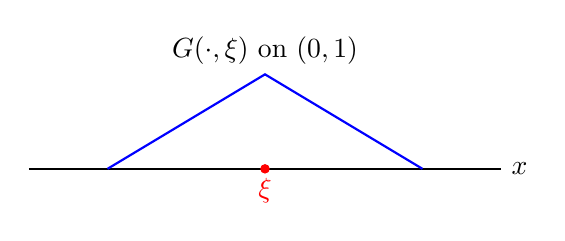
\begin{tikzpicture}[scale=1.0]
			\draw[thick] (-3,0)--(3,0) node[right] {$x$};
			\draw[thick,blue] (-2,0) -- (0,1.2) -- (2,0);
			\filldraw[red] (0,0) circle (1.5pt) node[below] {$\xi$};
			\node at (0,1.5) {$G(\cdot,\xi)$ on $(0,1)$};
		\end{tikzpicture}
		\caption{Schematic shape of a 1D Dirichlet Green function.}
	\end{figure}
	
\end{document}

